\documentclass{article}
\usepackage{amsmath, amssymb, ctex, graphicx, tasks}

\usepackage[margin=1in]{geometry}
\title{深度学习基础 - 概率 - 10个习题}
\author{《深度学习基础》课程小组}
\author{}
% \date{}

\usepackage{titling}
\setlength{\droptitle}{-2cm} % 标题上移

\begin{document}
\maketitle
% \tableofcontents

\textbf{2.2.} 
确定性数字满足\emph{传递性}属性，因此如果$x > y$且$y > z$，则可以得出$x > z$。然而，当我们转向随机数时，此属性不再适用。图2.16展示了一组按循环顺序排列的四个立方体骰子。证明这四个骰子中的每一个都有2/3的概率掷出比循环中前一个骰子更高的数字。这样的骰子被称为\emph{非传递性骰子}，这里显示的具体例子被称为\emph{埃夫龙骰子}。

\begin{figure}[ht]
    \centering
    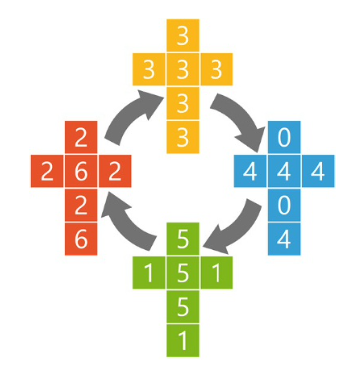
\includegraphics[height=5cm]{efron_dice.png}
    \caption{An example of non-transitive cubical dice}
    \label{fig:efron_dice}
\end{figure}


\textbf{2.3} 
考虑一个变量$\mathbf{y}$，它由两个独立随机变量的和给出，即$\mathbf{y} = \mathbf{u} + \mathbf{v}$，其中$\mathbf{u} \sim p_{\mathbf{u}}(\mathbf{u})$且$\mathbf{v} \sim p_{\mathbf{v}}(\mathbf{v})$。证明分布$p_{\mathbf{y}}(\mathbf{y})$由下式给出：
\begin{equation}
p(\mathbf{y}) = \int p_{\mathbf{u}}(\mathbf{u})p_{\mathbf{v}}(\mathbf{y} - \mathbf{u}) \,\mathrm{d}\mathbf{u}. \tag{2.119}
\end{equation}
这被称为$p_{\mathbf{u}}(\mathbf{u})$和$p_{\mathbf{v}}(\mathbf{v})$的\emph{卷积}。


\textbf{2.11} 
考虑两个具有联合分布$p(x, y)$的变量$x$和$y$。证明以下两个结果：
\begin{align}
\mathbb{E}[x] &= \mathbb{E}_y [\mathbb{E}_x[x|y]] \tag{2.122} \\
\text{var}[x] &= \mathbb{E}_y [\text{var}_x[x|y]] + \text{var}_y [\mathbb{E}_x[x|y]]. \tag{2.123}
\end{align}
这里$\mathbb{E}_x[x|y]$表示在条件分布$p(x|y)$下$x$的期望，条件方差也有类似的记号。


\textbf{2.16} 
均值为$\mu$、方差为$\sigma^{2}$的高斯分布，已知 $\mathbb{E}[x^2]=\mu^2+\sigma^2$, $var[x]=\sigma^2$. 
证明
\begin{equation}
\mathbb{E}\left[x_{n} x_{m}\right]=\mu^{2}+I_{n m} \sigma^{2}
\tag{2.128}
\end{equation}
其中$x_{n}$和$x_{m}$表示从均值为$\mu$、方差为$\sigma^{2}$的高斯分布中采样的数据点，并且$I_{nm}$在$n=m$时满足$I_{nm}=1$，否则$I_{nm}=0$。


\textbf{2.19} 
利用概率密度在变量变换下的变换性质(2.71)，证明任何密度$p(y)$都可以通过对一个处处非零的固定密度$q(x)$进行非线性变量变换$y=f(x)$来获得，其中$f(x)$是一个单调函数，使得$0 \leqslant f^{\prime}(x)<\infty$。写出$f(x)$所满足的微分方程，并绘制一个图示来说明密度的变换。

\textbf{2.20} 
计算由
\begin{align}
y_1 &= x_1 +\tanh(5x_1), \\
y_2 &= x_2 +\tanh(5x_2) +\frac{x_1^3}{3} 
\end{align}
定义的变换的雅可比矩阵的元素。


\textbf{2.25} 
证明单变量高斯分布$N(\mu,\sigma^2)$的熵由下述给出：
$$
H[x]=\frac{1}{2}(1+\ln (2\pi\sigma^2)).
$$

\textbf{2.27} 
计算两个高斯分布$p(x)=\mathcal{N}\left(x | \mu, \sigma^{2}\right)$和$q(x)=\mathcal{N}\left(x | m, s^{2}\right)$之间的Kullback-Leibler散度。

\textbf{2.29} 
考虑两个具有联合分布$p(\mathbf{x}, \mathbf{y})$的变量$\mathbf{x}$和$\mathbf{y}$。证明这对变量的微分熵满足
\begin{equation}
\mathrm{H}[\mathbf{x}, \mathbf{y}] \leqslant \mathrm{H}[\mathbf{x}]+\mathrm{H}[\mathbf{y}]
\tag{2.130}
\end{equation}
当且仅当$\mathbf{x}$和$\mathbf{y}$统计独立时取等号。

\textbf{2.30} 
考虑一个具有分布$p(\mathbf{x})$和相应熵$\mathrm{H}[\mathbf{x}]$的连续变量向量$\mathbf{x}$。假设我们对$\mathbf{x}$做一个非奇异线性变换以获得一个新变量$\mathbf{y}=\mathbf{A} \mathbf{x}$。证明相应的熵由$\mathrm{H}[\mathbf{y}]=\mathrm{H}[\mathbf{x}]+\ln \operatorname{det} \mathbf{A}$给出，其中$\operatorname{det} \mathbf{A}$表示$\mathbf{A}$的行列式。

\textbf{2.31} 
假设两个离散随机变量$x$和$y$之间的条件熵$\mathrm{H}[y | x]$为零。证明对于所有满足$p(x)>0$的$x$值，变量$y$必须是$x$的函数。换句话说，对于每个$x$，只有一个$y$值使得$p(y | x) \neq 0$。


\textbf{2.36} 
考虑两个具有如下联合分布的二元变量$x$和$y$：
\[
\begin{array}{c|cc}
 & \multicolumn{2}{c}{y} \\
x & 0 & 1 \\
\hline
0 & 1/3 & 1/3 \\
1 & 0 & 1/3 \\
\end{array}
\]
计算以下量：
\begin{tasks}(3)
\task $\mathrm{H}[x]$
\task $\mathrm{H}[y]$
\task $\mathrm{H}[y|x]$
\task $\mathrm{H}[x|y]$
\task $\mathrm{H}[x, y]$
\task $\mathrm{I}[x, y]$.
\end{tasks}
绘制一个维恩图来展示这些不同量之间的关系。

\textbf{2.38} 
利用概率的加法和乘法规则，证明互信息$I(\mathbf{x}, \mathbf{y})$满足关系式
$$
I(x,y) = H(x) - H(x|y) = H(y) -H(y|x). 
$$

\textbf{2.40} 
考虑图2.2中的弯曲硬币。假设凸面朝上的先验概率为0.1。现在假设将这枚硬币抛掷10次，并被告知其中有8次正面朝上，2次反面朝上。使用贝叶斯定理评估凹面朝上的后验概率。计算下一次抛掷正面朝上的概率。


\end{document}

